\documentclass[10pt]{article}%added to see figs (also changes caption
								%placement and format)
%\bibliographystyle{naturemag}
\usepackage{graphicx} %added to view pics
\usepackage{lineno} %added to see line numbers
\usepackage[fontsize=9]{scrextend} %added to allow for small fonts
\usepackage{color,soul} %added for highlighting text, use \hl{}

\begin{document}
\title{BICXS Data Analysis}
\maketitle

\tableofcontents 

\section{Introduction}
We developed a more robust methodology to determine level of interaction between biomolecules than other current techniques by use of molecular probes and the analysis of their SAXS data. Molecular probes are attached to each player in the interaction and are assumed to be interacting when the probes are in close proximity to each other. Determining the approximate distances between probes in bulk solutions will not only give indications as to the level of interaction, but also the likely conformation of the interacted biomolecules. This document explains how to derive this information from the experimentally measured SAXS profiles.

\subsection{Experimental Protocol}
The protocol is to measure the sample, the background of the sample (often times the buffer), a dark frame, and a beam profile. Rows of pixels were binned along the slit length so that the effective pixel sizes were larger and collects more photons in a shorter amount of time allowing us to collect more signal while keeping noise low. Moreover, multiple frames were captured for every SAXS measurement and averaged to reduce effects of cosmic ray radiation and random noise from other effects.

% Should I tabulate the energy, # of frames, length of exposure per frame here?
 
The Anton Paar SAXSpace system accompanied software, SAXSdrive (Ashland, VA), acquires and outputs each experiment data in  conventional three column data: scattering angle ($q$~[$nm^{-1}$]), scattering intensity ($I_{exp}$~[$a.u.$]), and standard deviation ($\sigma [a.u.]$). 

\section{Basic SAXS Data Analysis}
A brief overview of common data analysis techniques are documented here. 

\subsection{Preliminary Data Treatment}
This section contains information on how to treat the data outputted from the SAXS instrument to a workable format. 

\subsubsection{Box and $\pi$ Averaging}
to be considered for another paper... (proposal)

\subsubsection{Conversion of detector pixels to scattering angle}
SAXSdrive outputs the data in terms of scattering angle ($nm^{-1}$), however the considerations are listed below.  
\begin{figure}[ht]
\centering
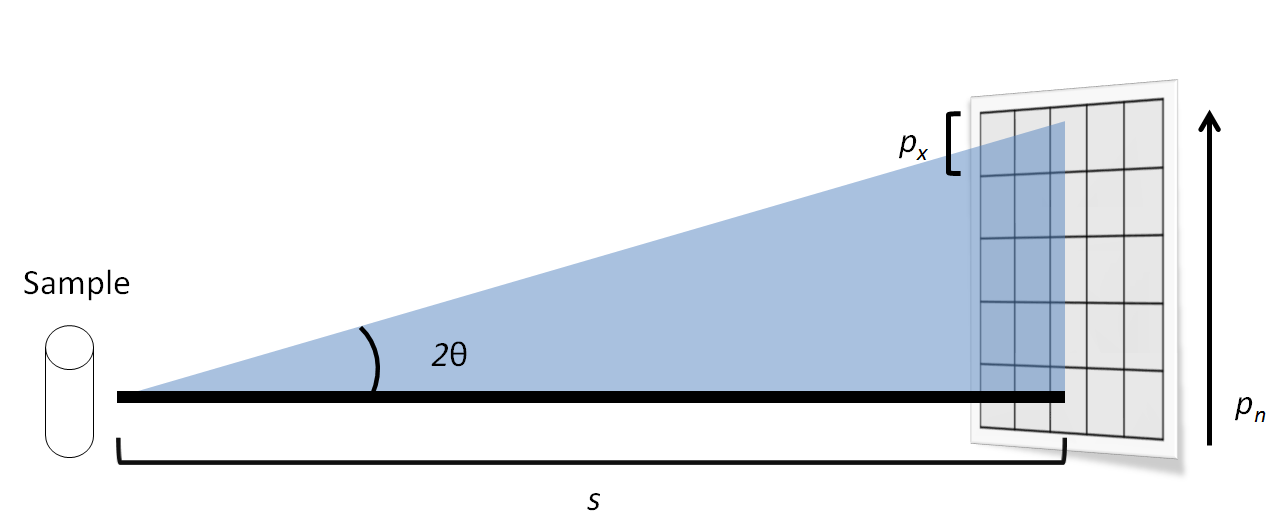
\includegraphics[scale=.35]{images/pixel2q_diagram.png}
\caption{Diagram relating variables to the equations converting pixels to scattering angle, $q$.}
\label{pixel2q}
\end{figure}

\begin{equation}
\lambda= \frac{hC}{E}
\end{equation}
where $\lambda$ is the x-ray wavelength, $h$ is Plank's Constant, $C$ is the speed of light, and $E$ is energy of the x-ray source.

\begin{equation}
2\theta=arctan \frac{p_x p_n}{s}
\end{equation}

where $p_x$ is the pixel pitch, $p_n$ is the pixel number from the primary beam, $s$ is the sample-to-detector distance in $nm$. See Fig.~\ref{pixel2q} for diagram reference on variables.  

\begin{equation}
q=\frac{4 \pi sin(\theta)}{\lambda}
\end{equation}

\subsubsection{Subtraction}
If we define noise as anything other than the signal of interest (scattering intensity from the GNP), subtraction is a way for us to remove noise caused by the electronics and other scatterers along the beam path. The protocol is to measure the sample, then measure the background of the sample (often times the buffer) in the exact same acquisition settings and sample holder ($1~mm$ diameter quartz capillary). 
To get a better subtraction of the data, effects caused by minor movements in the collimation system, and beam stop position were minimized by acquiring all data for subtraction on the same day immediately after (or before) measurement of the sample.  

A dark measurement was subtracted from the sample and background intensity measurements to reduce noise from dark current and other errors from hot or stuck pixels that often occur due to long exposure times. 

For each sample of interest, the scattering intensity of the buffer must be acquired for better background subtraction. The buffer in our experiments was deionized water. 

\begin{figure}[ht]
\centering
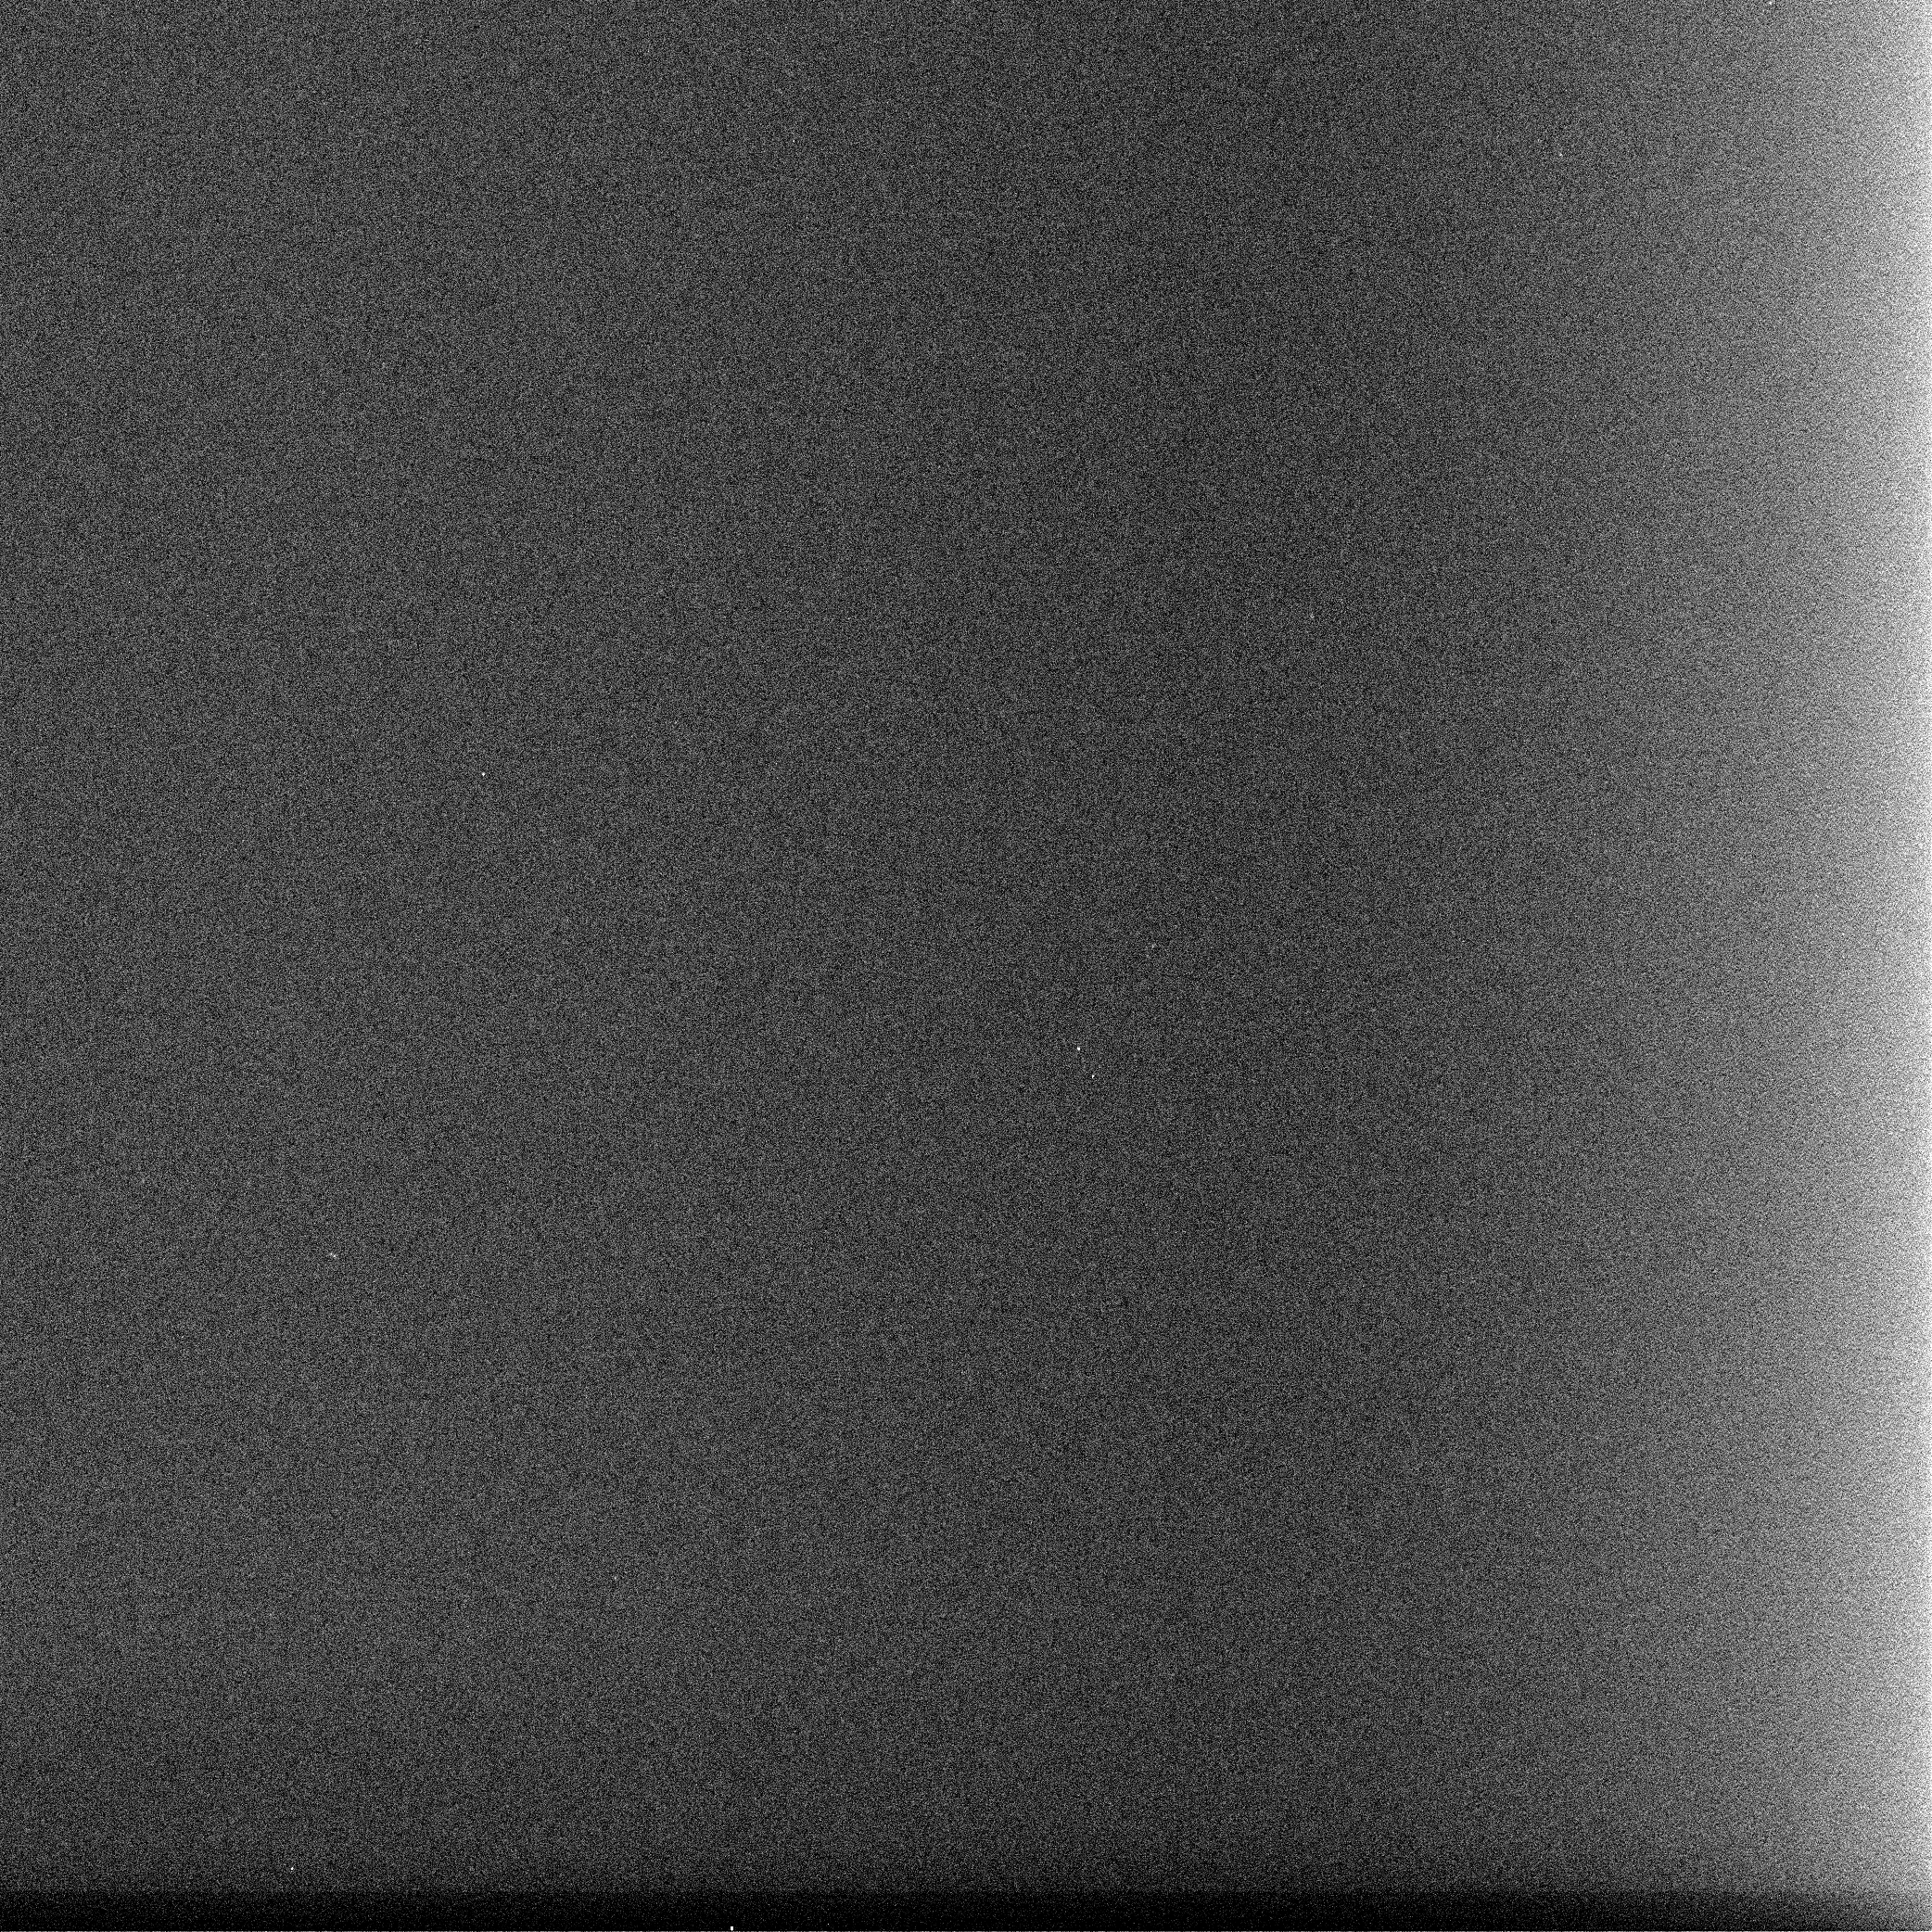
\includegraphics[width=5cm]{images/darkcurrent2.png}
\caption{Dark frame. \textit{Note:} Windowing and levelling was performed on the image to accentuate the uneveness in the pixel intensities.}
\end{figure}
\begin{equation}
I_{SOI}^{-}=(I_{SOI}-I_{dc}).*f - (I_{bg}-I_{dc})
\end{equation}

$f$ is a relative transmittance scaling factor that is often necessary when the sample's absorption of x-rays is greater than the background absorption. If the sample absorbs more x-rays, the scattering intensity will be less than the background, and thus, the subtraction will result in unusable negative numbers. Unfortunately, exact transmittance of sample and the background are not always available. For practical reasons, $f$ can be estimated by setting a value that will set $I_{SOI}$ at or as close as possible to the $I_{bg}$ at wider scattering angles where the scattering effect of dispersed sample particles are no longer significant and should be the same in the background. If $f$ is equal to 1, dark frame subtraction is redundant as the dark current effects will be taken care of in the background subtraction. 


SAXSdrive outputs the data already in terms of the scattering angle, $q$, however, the scattering angle relates to pixels in the equations below. 

\subsubsection{Data Reduction}
The scattering profile from all measurements include a fraction of the primary beam that have transmitted through the beam stop. All measurements are $q$ calibrated so that the location of the primary beam is the zero scattering angle. In Fig.~\ref{datareduction}, the first peak for both the sample and the background curves show the primary beam, and the second peak is the scattering information starting from the edge of the beam stop and ending when scattering information is hidden beneath the noise floor. The noise floor is more apparent after subtraction and when plotted using a log-scale y-axis. The useful region of data for subsequent sections is from that edge of the beam stop to the noise floor. It is important to reduced the edges of the data to get an optimized data fitting in later sections.
     
\begin{figure}[h]
\centering
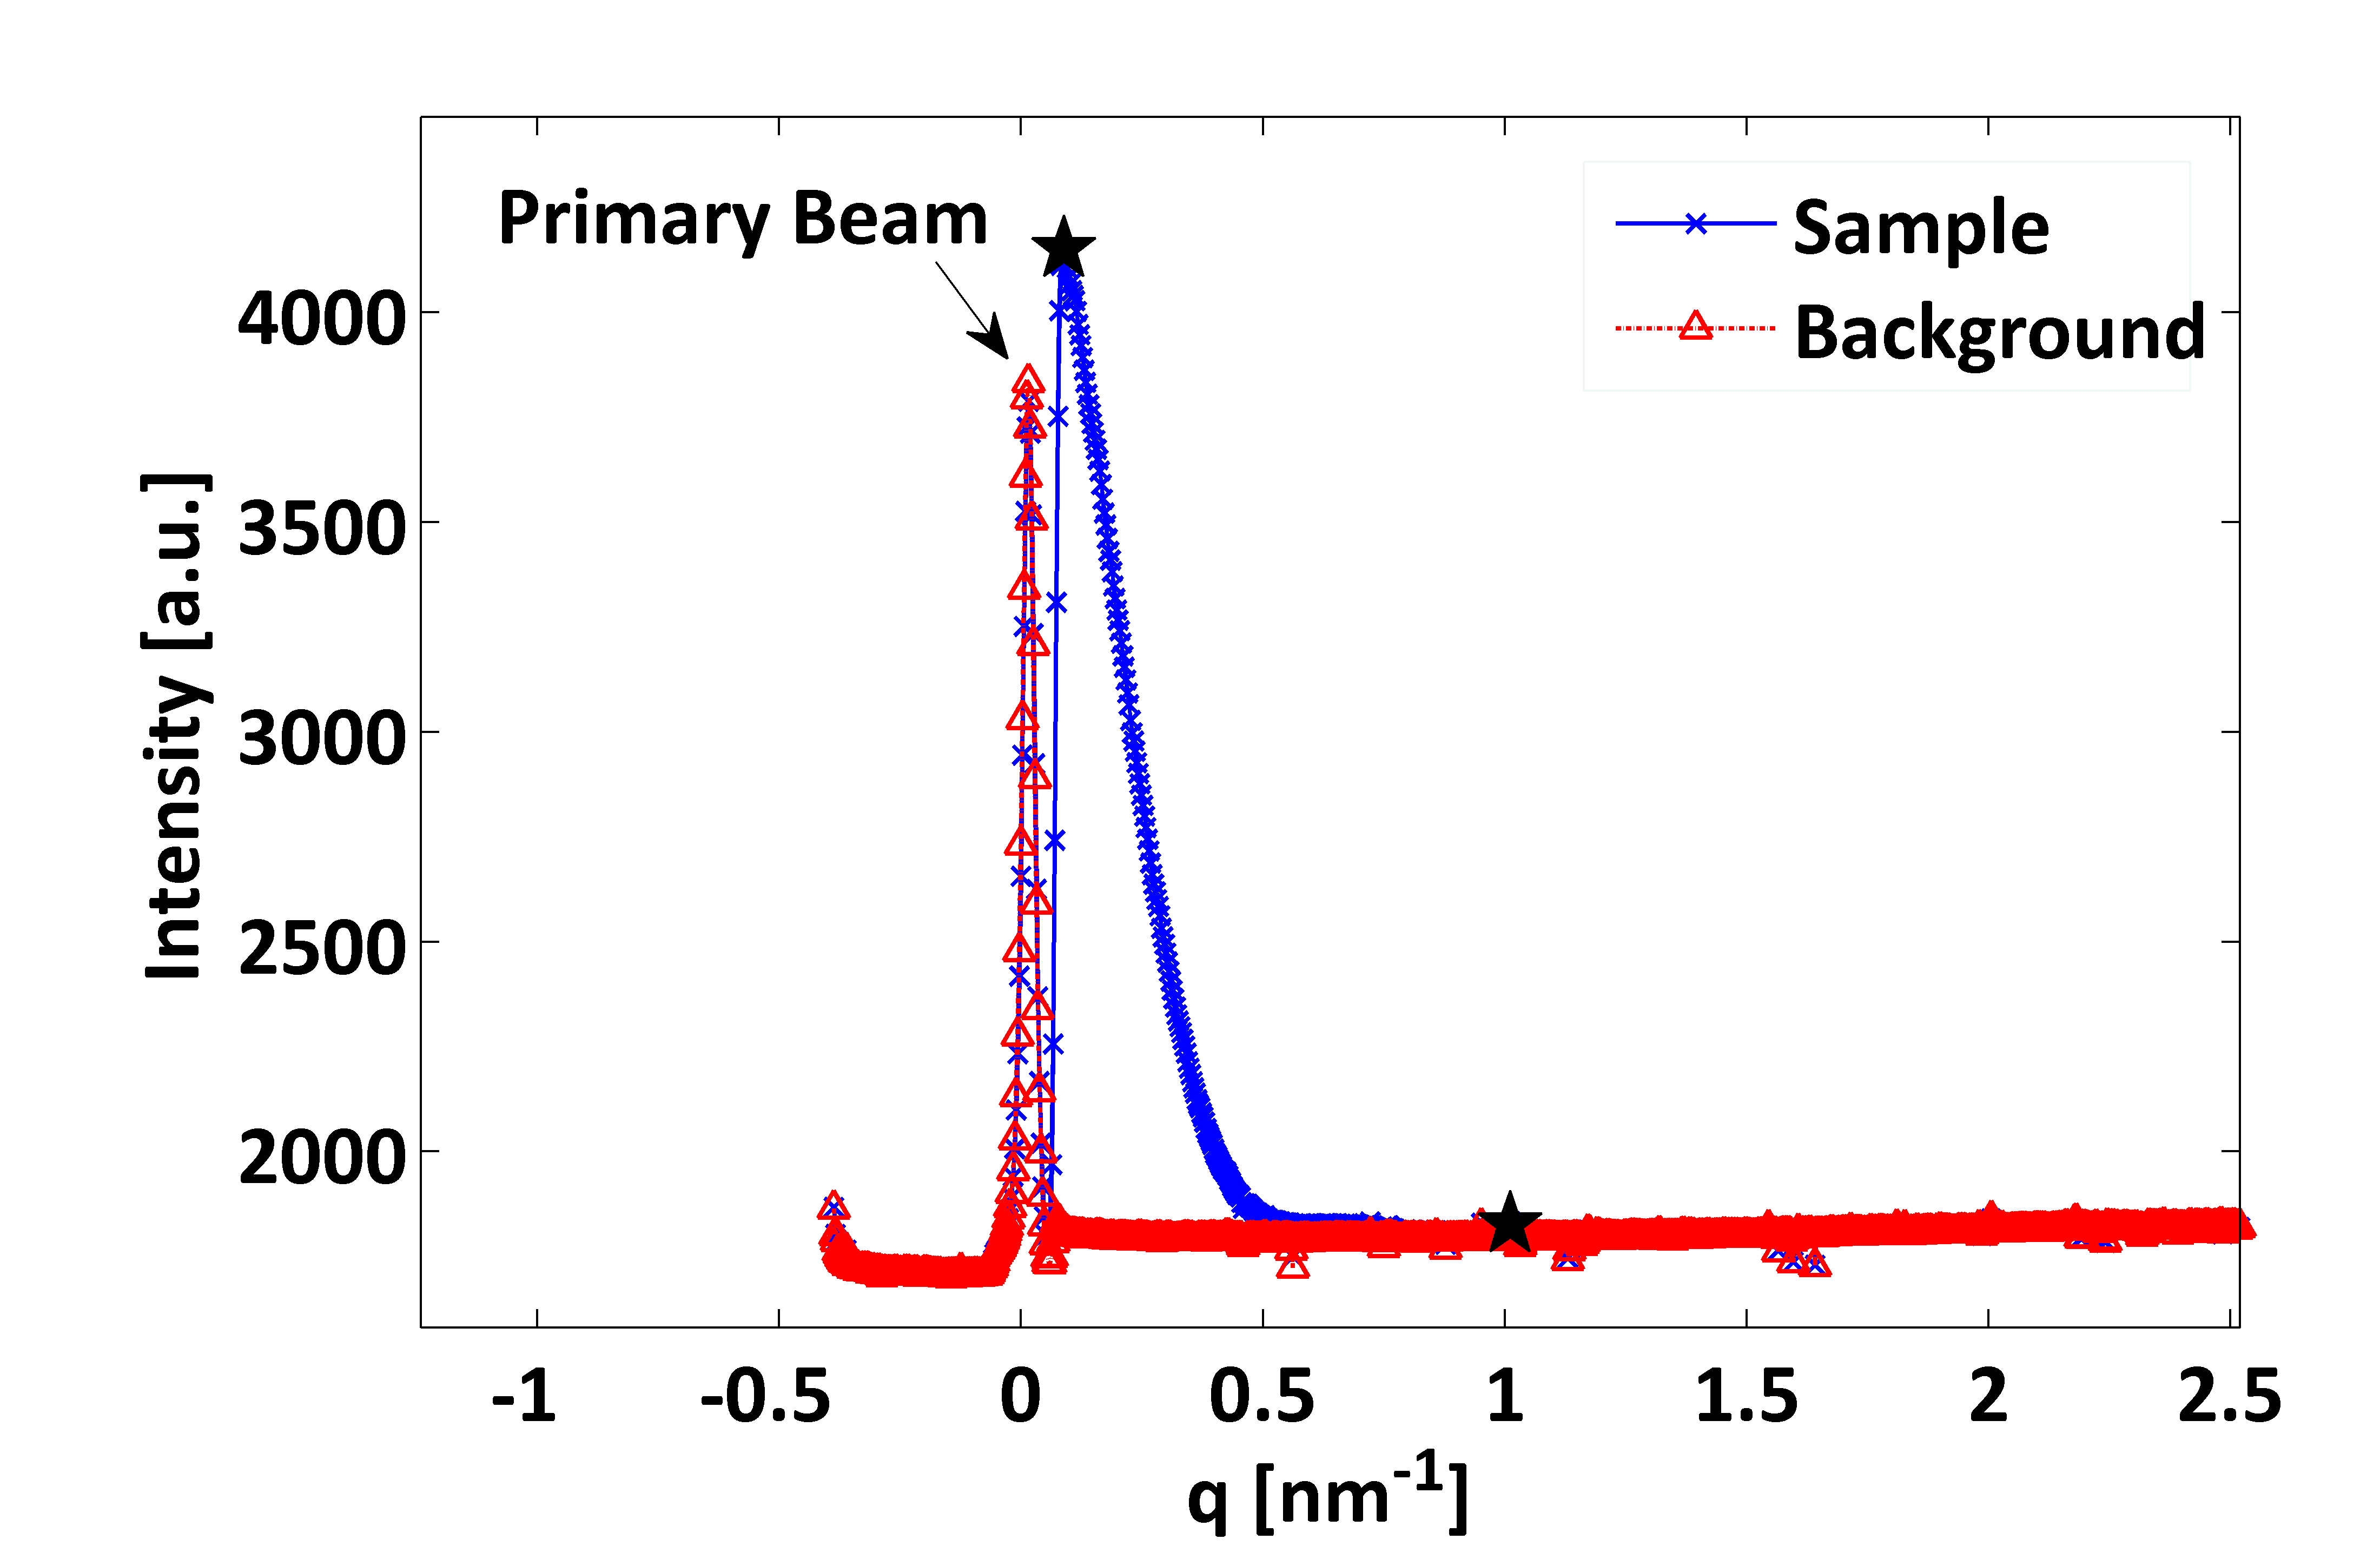
\includegraphics[scale=.5]{images/datareduction.png}
\caption{The data between the black stars indicate the a usable and informative region of interest in the scattering profile. The primary beam peak is necessary to detect where $q=0$.}
\label{datareduction}
\end{figure}



%%
A dark measurement was subtracted from the sample and background intensity measurements.

\begin{equation}
I_{sample*}=(I_{sample}-I_{dc})f - (I_{bg}-I_{dc})
\end{equation}

$f$ is a relative transmittance scaling factor that can be estimated by setting a value that will set $I_{sample}$ at or as close as possible to the $I_{bg}$ at wider scattering angles.

The scattering profile from all measurements include a fraction of the primary beam that have transmitted through the beam stop. All measurements are calibrated so that the pixel position of the primary beam is the zero scattering angle. 

\subsection{Beam Profile}
Our measurements were taken using a line collimated system, more specifically, a Kratky-block collimation. A beam profile was obtained after every alignment of the SAXS system. A trapezoidal fit was used to fit the beam length profile for the smearing and desmearing processes. Beam width and wavelength effect were negligible. The equation used is as follows that ignores the wavelength and slit width effect but accounts for beam length. 

\begin{equation}
I_m(h)=8\pi\int_0^{\infty}dr\int_0^{\infty}dt \times P(t)p(r)sin(\beta)/\beta 
\end{equation}

where $\beta=r\sqrt{h^2+t^2}/\lambda_0$. P(t) is centered at zero and scaled such that $\int_P P(t) dt=1$. $t$ is in $nm^{-1}$.

\subsection{Indirect Fourier Transform (IFT)}
IFT is used to convert the data from spatial frequency $I(q)$ to real space $p(r)$. From this process, we also get a smoothed fit of the data by use of weights that are solved to obtain $p(r)$.

In our custom implementation of IFT, we use 20 splines and each of our splines are $1~nm$ in full-width half maximum (FWHM) between 0 and $D_{max}$ which is defined to be the \textit{a priori} knowledge or estimate of the longest pair-distance in the particle. Any value beyond $D_{max}$ is set to zero. 

We use 17 different alpha values evenly distributed between $10^{-4}$ and $10^5$ which have been sufficient in finding the appropriate stabilization parameter, $\alpha$, the point at which the $N_c''$ has plateaued and the point before the mean deviation (MD) exponentially increases. The fit is considered good when $MD$ is approximately equal to 1.0. 

\section{Modelling Dimers}

\begin{figure}
\centering
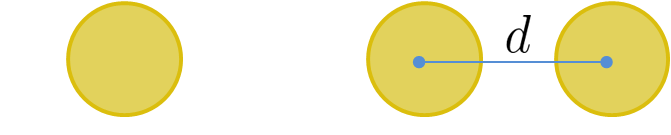
\includegraphics[scale=.3]{images/diagram.png}
\caption{A pictoral representation of the gold nanoparticle monomer and dimer.  The dimer is defined to be two GNP monomers $d$ distance apart from center-to-center. Not shown is the proteins and/or biomolecules that bind the two GNP monomers because the scattering from the biomolecules is small compared to the scattering from the GNP and is essentially hidden in SAXS measurements.}
\end{figure}

For any scatter from a monodisperse object, we can dimerize the scattering intensity analytically by applying Eq.~\ref{dimerize} \ref{kaya04apr}.

\begin{equation}
I_{dimer}=I_{monomer}(2+2\frac{sin(qd)}{qd})
\label{dimerize}
\end{equation}

\subsection{Smearing}
In order to compare a smeared experimentally measured monomer scatter profile with an analytically solved dimer scatter profile, we must also smear the dimer scatter profile. See Fig.~\ref{dimerflow} for a flow diagram of how we solve for a smeared dimer scatter profile. 

\begin{equation}
I^{*} =\int_P P(t) I(\sqrt{(q)^2+t^2}) dt 
\label{smear}
\end{equation}

Eq.~\ref{smear} analytically smears the scatter profile, $I$, based on a beam profile, P(t). $*$ is used to denote smeared. 
\section{Quantifying Interaction Levels}

\begin{figure}
\centering
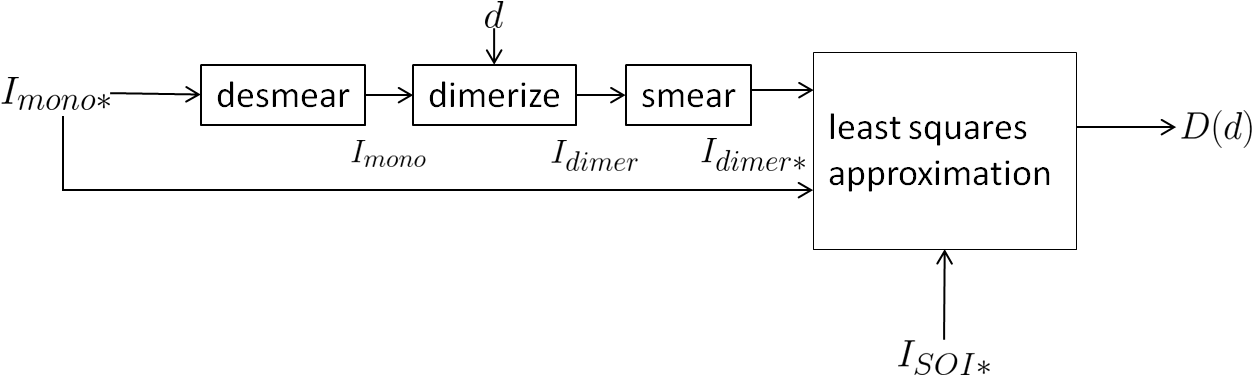
\includegraphics[scale=.5]{images/flowdiagramlevel2.png}
\caption{Flow diagram of how to dimerize our experimentally measured monomer scatter. For point-collimated data, the desmearing and smearing steps can be disregarded. $*$ is used to denote experimentally obtained or smeared data. $I_{SOI}$ is the scattering intensity of the sample of interest that we are determining the fraction of interacting particles.}
\label{dimerflow}
\end{figure}

Given an experimentally measured and treated monomer GNP probe scattering data, $I_{monomer}$, and measured and treated data of a sample of interest that contains both monomers and dimers depending on interaction level of the proteins and linkers attached to the monomers, $I_{SOI}$, we estimate the fraction of monomers to dimers and the approximate distance between monomers in the interacting particles.
First, the monomer sample scatter data is fitted using \textit{IFT}, then the smoothed monomer scatter function is \textit{dimerized} analytically using several $d$ values. Since our monomer is known to be $10~nm$ in radius, the minimum $d$ was set to $20$ and the maximum was set to $60$ with increments of $1$. This series of dimerized scatter functions is $I_{dimer(s)}$. The $I_{monomer}$ and $I_{dimer(s)}$ are placed in a matrix, $C$.  The unaltered $I_{SOI}$ scatter profile is approximated using a non-negative least squares fit with $C$.  The result are weights, $x$, for each of the functions in $C$ that give an estimate as to the distribution of monomers to different $d$ dimers in the mixed sample.

\begin{equation}
min_x ||C\dot x- I_{SOI}||^2_2,\hspace{.5 cm} where \hspace{.2 cm} x \le 0
\end{equation}


%\bibliographystyle{plain} 
{\footnotesize\bibliography{sharedbib}} 

\end{document}
